\begin{figure} [H]
	\centering
	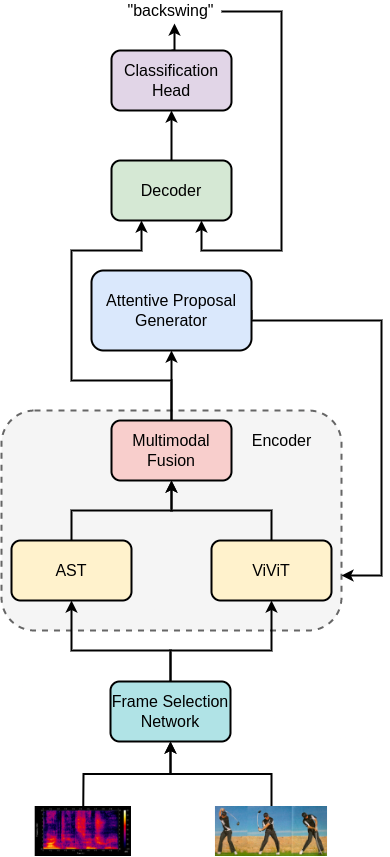
\includegraphics[width=7cm, height=12cm] {assets/img/dvc_arch.png}
	\caption{Proposed model for Dense Video Captioning}
\end{figure}

\subsection{Multimodal Feature Extraction}
\par Feature extraction is the backbone of our solution to tackle the task of Dense Video Captioning \cite{krishna2017densecaptioning}. A rich feature space would enhance the representational power of the model, thereby leading to more meaningful and accurate event proposals. Most previous works have utilized one modality only (i.e. video) to generate feature vectors as input to the proposal generator. However, audio cues, in conjuction with video is a strong event indicator. These events are accompanied with a sharp change in their corresponding audio spectogram which can be learnt by the model to better determine the precise boundary of events. Thus, we aim to combine features generated using both video and audio. Currently, we are exploring two methods of fusion which include the cross-attention mechanism \cite{iashin2020better} and common space proejction using contrastive learning \cite{vatt}.


\subsubsection{Video Features}
\par Video features are the most important part of the encoder. Without a robust and rich feature space for videos, the proposal generator would never be able to learn accurate event boundaries. Previous state-of-the-art video encoders \cite{carreira2018quo}, \cite{csn}, \cite{r(2+1)d} use CNN-based architectures. Although they have strong inductive bias and translational invariance, they fail to model long-range temporal dependencies which are of paramount importance when encoding videos. Moreover, CNNs require different architectures to model different modalities which can become complex when combining multiple modalities such as video and audio. Transformers \cite{tfm} can overcome these barriers using its attention mechanism without comprimising on its statistical and computational efficiency. Moreover, transformers can use the same building blocks across different modalities without many modifications. We aim to use the recently proposed ViViT model \cite{vivit}, a purely attention-based video encoder which has outperformed previous approaches across several datasets such as  Kinetics 400 and 600, Epic
Kitchens 100, Something-Something v2 and Moments in Time. Even though ViViT requires several orders of magnitude more training data as compared to its CNN counterparts, the authors of ViViT propose several methods to limit its training by using pretrained weights in conjunction with strong regularisation and specific fine-tuning. 

\begin{figure} [H]
	\centering
	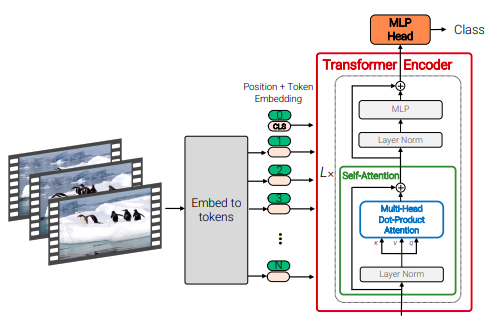
\includegraphics[width=7cm, height=6cm] {assets/img/vivit_methodology.png}
	\caption{ViViT encoder by Dosovitskiy \textit{et al}. (Image courtesy \cite{vivit})}
\end{figure}

\subsubsection{Audio Features}
\par Audio is an important aspect of any video. Not only does audio suggest the duration of an event, it can also signify the magnitude or significance of that event. Thus, audio becomes a powerful accessory to images when representing a video. We aim to use the recently proposed Audio Spectogram Transformer (AST) \cite{ast} which has outperformed current state-of-the-art models in audio classification. Moreover, AST uses pretrained weights from ViT \cite{vit}, just like ViViT. We believe that this would thus, work cohesively with ViViT and lead to richer multimodal features.

\begin{figure} [H]
	\centering
	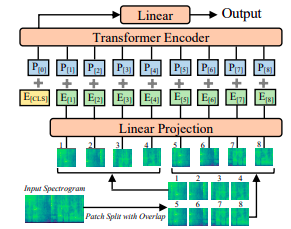
\includegraphics[width=7cm, height=6cm] {assets/img/ast_methodology.png}
	\caption{AST encoder by Gong \textit{et al}. (Image courtesy \cite{ast})}
\end{figure}

\subsection{Training}
\subsubsection{Knowledge Distillation}
\par We aim to use the Knowledge Distillation framework (student-teacher paradigm) to train the model, either in individual modules or as a whole. For the video encoder (ViViT), we would use a strong CNN-based video classifier as the teacher model to introduce inductive bias within the transformer and reduce training.Touvron \textit{et al} introduced a method for knowledge distillation \cite{deit} using a distillation token to compute the loss based on the softmax generated by the teacher model. 
\par We also aim to train the proposal generator using a student-teacher paradigm with the current SOTA DVC models. 

\begin{figure} [H]
	\centering
	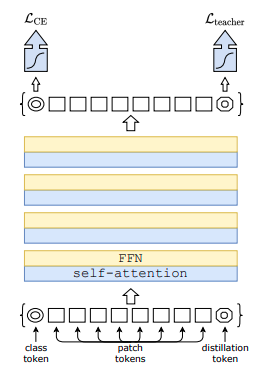
\includegraphics[width=6cm, height=9cm] {assets/img/deit.png}
	\caption{Distillation through attention by Touvran \textit{et al}. (Image courtesy \cite{deit})}
\end{figure}
